\documentclass[conference]{IEEEtran}
\IEEEoverridecommandlockouts
% The preceding line is only needed to identify funding in the first footnote. If that is unneeded, please comment it out.
\usepackage{cite}
\usepackage{amsmath,amssymb,amsfonts}
\usepackage{algorithmic}
\usepackage{graphicx}
\usepackage{hyperref}
\usepackage{listings}
\usepackage{minted}
\usepackage{textcomp}
\usepackage{xcolor}

\def\BibTeX{{\rm B\kern-.05em{\sc i\kern-.025em b}\kern-.08em
    T\kern-.1667em\lower.7ex\hbox{E}\kern-.125emX}}
\begin{document}

\title{Nature-Inspired Computing\\Project Report\\}

\author{\IEEEauthorblockN{Ayhem Bouabid}
\IEEEauthorblockA{\textit{DS-01} \\
\textit{Innopolis University}\\
Innopolis, Russian Federation \\
a.bouabid@innopolis.university}
\and
\IEEEauthorblockN{Majed Naser}
\IEEEauthorblockA{\textit{DS-01} \\
\textit{Innopolis University}\\
Innopolis, Russian Federation \\
m.naser@innopolis.university}
\and
\IEEEauthorblockN{Nikolay Pavlenko}
\IEEEauthorblockA{\textit{DS-01} \\
\textit{Innopolis University}\\
Innopolis, Russian Federation \\
n.pavlenko@innopolis.university}
}

\maketitle

\begin{abstract}
Preprocessing and dataset optimization play an important role in machine learning models. Nature-inspired algorithms such as particle swarm optimization, genetic algorithm and cuckoo search algorithm can be creatively combined into a preprocessing pipeline that will rid the dataset of uninformative features and transform the data without harming the predictive capacity of the model.
\end{abstract}

\begin{IEEEkeywords}
multicollinearity, clustering, nature-inspired algorithms, particle swarm optimization
\end{IEEEkeywords}

\section{Introduction}

The initial goals that we have set in this project was applying nature-inspired algorithms as optimizers to the dataset that contained various features that were supposed to predict population growth. The resulting dataset would be evaluated by regression Machine Learning (referred to as ML) models, and results of our preprocessing would be evaluated. However, after starting working on the project, it very soon became evident that the project would have had a very small scope, and few opportunities to explore interesting applications of Nature Inspired Algorithms (referred to as NIA). \\ 

Therefore, our final project represents a significant extension of the initial proposal. The latter constitutes of predicting the population’s growth using a combination of Machine Learning and Nature Inspired Computing techniques (referred to as NIC). The final project takes this first \emph{\textbf{experimental}} step into a more complex and sophisticated direction. Our team attempts to build a ML preprocessing pipeline almost fully-based on NIC techniques and evaluates its performance with the considered dataset as per with the initial proposal. Such direction was motivated by a number of considerations including:
\begin{enumerate}
	\item The performance of ML models is highly correlated with the quality of the data fed to the algorithms. Performing feature selection allows us to solve a great number of problems, being especially effective in large datasets containing many features. It improves accuracy of predictions by finding and eliminating spurious relationships, as well as reducing the chances of overfitting. Other effects of feature selection are the improvement of training time for the model through cutting down on unnecessary data, and increase in interpretability, as fewer features have to be analyzed to figure out the dependencies. Therefore, Feature engineering as well as data preprocessing represent pillars of a high-performing end-to-end ML pipeline.
	\item Although data preprocessing, manifested mostly in feature selection, represents one of the main applications of NIC algorithms, \textbf{feature engineering} on the other hand has not received its fair share of the scientific community’s attention. The \emph{art} of feature engineering, as mentioned above, is a crucial step of Machine Learning pipelines and an extremely valuable skill for each and every ML practitioner. Our project attempts to build an NIC-based framework for two major “feature engineering techniques”:
	\begin{itemize}
		\item Eliminating multicollinearity
		\item Feature transformations
	\end{itemize}
	\item If we succeed in developing preprocessing that will efficiently reduce the number of features in the initial dataset, the pipeline that we developed will have to be tested on other similar datasets in order to demonstrate its effectiveness. The problem of predicting population growth covers a lot of the same variables that would be useful in predicting other statistics important in banking, finance, or government, so if our model proves its effectiveness on a more generic dataset, its area of applicability will expand significantly.\\
	
\end{enumerate}

With that goal in mind, during the testing process we have resorted several times to generating new datasets (both for regression and classification problems) with the help of tools provided by the sklearn libraries, with randomly assigned or manually set parameters.\\
	
Our project will have the following structure:
\begin{enumerate}
	\item Data Preparation
	\item Multicollinearity Reduction using \textbf{Particle Swarm Optimization} algorithm
	\item Feature selection with \textbf{Cuckoo Search} algorithm
	\item Feature transformations with \textbf{Genetic Algorithms}
	\item Additional minimalistic preprocessing of the dataset and comparison of a number of ML models performances with and without our experimental pipeline.
\end{enumerate}

\section{Related Work}

The idea of feature selection using Nature-Inspired Algorithms is not new - we have based our project around already existent frameworks that implement those algorithms and apply them as optimizers in preprocessing tasks.\\

One framework that we have used in our project is NiaPy library\cite{niapy}. They have implemented a large collection of nature-inspired algorithms, and provided a simple interface to use them as optimizers. Their library is also used by the Transaction Fraud Detection project, which is based around the same idea of feature selection with the nature-inspired algorithms and has served as an inspiration behind our own project, so we have decided to follow in their footsteps.\\

Later, in the process of searching for another library that is compatible with NiaPy implementation of various nature-insipred algorithms, and would provide a friendly and extendable Python interface to use them as optimizers in combination with Pandas and sklearn libraries, we have found the evopreprocess library\cite{evopreproc}. \\

That library contains several main modules: \texttt{data\_sampling}, \texttt{data\_weighting}, and \texttt{feature\_selection}. Howeveer, only the last module is relevant for our task, so we will only describe its functionality. The task class for \texttt{feature\_selection} in evopreprocess is \texttt{EvoSampling}, which extends \texttt{\_BaseFilter} class from scikit-learn. It is important to list the parameters of that class, as they are going to play a big role in the feature selection process:
\begin{itemize}
	\item \texttt{random\_seed} - seed state, by default is equal to system time in milliseconds.
	\item \texttt{evaluator} - ML approach used to evaluate the data, expecting a scikit-learn-compatible regressor or classifier.
	\item \texttt{optimizer} - NI optimizer, expecting a NiaPy-copatible method, by default Genetic algorithm
	\item \texttt{n\_folds} - number of folds for the cross-validation split into training and validation sets
	\item \texttt{n\_runs} - number of runs of the optimizer on each fold
	\item \texttt{benchmark} - evaluation class that measures the quality of data sampling. By default optimizes error rate and F-score for classification problems and mean square error for regression problems
	\item \texttt{n\_jobs} - number of optimizers to be run in parallel, by default equal to the number of your CPU's cores
\end{itemize}

\section{Methodology}

\subsection{Data preparation}

The population’s growth dataset was built upon the different datasets made available by the “world bank of data”\cite{world_bank_moment}. In this regression problem, models are predicting the annual demographic growth based on features covering a country’s significant statistics\cite{kelley1973population}\cite{sinnathurai2013empirical}, such as: 
\begin{enumerate}
	\item Population: age, dependency ratio, etc.
	\item Agriculture: annual food production, etc.
	\item Health: mortality rate, etc.
	\item Education: percentage of school enrollment, etc.
\end{enumerate}

Furthermore, some inputting and interpolation methods were applied, such as:
\begin{itemize}
	\item Spline - efficient for inputting piece-wise changeing of variables, it preserves the seasonality in data.
	\item Linear - based on the assumption that the datapoints are linearly spaced in time, as is likely for the type of data that we collect.	
\end{itemize}

\subsection{Multicollinearity issue}

\subsubsection{Problem description}

Before describing our approach to solve the \textbf{multicollinearity} problem, it is of significance to better describe the statistical phenomena. Mutlicollinearity manifests itself when one or more predictors (features) can be predicted with high accuracy using the other predictors. This statistical phenomena leads to several issues:

\begin{itemize}
	\item The coefficients computed by linear models can be sensitive even to small changes in the data, leading to significant generalization error
	\item The model's interpretability and estimation of features' importance suffers, as is the case with one of the most robust ML models: random forest\cite{sklearn_permutation}.	
\end{itemize}

\subsubsection{Multicollinearity detection}

Multicollinearity can be detected in a dataset by finding the VIF - variance inflation factor, calculated for each feature separately, according to the formula below, where $R^2$ is the coefficient of determination: 

\begin{equation}
	VIF=\frac{1}{1-R^2}
\end{equation}

VIF can normally take positive values, and by checking its value for each column, one could determine whether or not a serious issue is detected. According to some authors, value of VIF greater than 1 identifies existence of some collinearity, greater than 5 is already a cause for concern, and greater than 10 must be addressed. However, in our solution we have selected 2.5 as a boundary for VIF, as a low boundary allows us to include more features in clusters and make the results of application of our method more evident.\cite{menard2002applied}.\\

As our solution to multicollinearity we have decided to combine 2 techniques: clustering and Particle Swarm Algorithm.\\

\subsubsection{Clustering}

Our solution is inspired by the following approach that is presented in the sklearn documentation\cite{sklearn_permutation}:
\begin{enumerate}
	\item Consider the Spearman correlation as a distance measurement.
	\item Build hierarchical clustering using Ward's clustering algorithm.
	\item Determine a threshold for cutting the resulting dendogram.
	\item Group the features according to the remaining clusters and keeping a single feature out of every group.	
\end{enumerate}

\subsubsection{Particle Swarm Optimization Clustering}

Particle Swarm Optimization is one of the most influential Nature-Inspired algorithms that can optimize a problem by iteratively improving a chosen solution, depending on the elected performance measure\cite{ballardini2018tutorial}. This property makes it possible to use PSO for our clustering problem, where the final choice of solution will be determined by the algorithm and defined fitness function. The solutions to our optimization problem will be represented as particles, and the aim of the algorithm will be to adjust those particles' position according to the best one found so far, and the best position in the neighborhood of that particle.\\

where $N_c$ is umber of clusters in the particle, $C_i$ is set of features belonging to i-th cluster, $f_i$ is i-th feature as a vector.\\

Implementation of PSO that we used in our work has specific important parameters, the values we assigned to them as well and the reasoning behind those assignments are listed below:
\begin{itemize}
	\item \texttt{func} - contains the function that PSO will be trying to optimize, in our case is equal to the cluster scores
	\item \texttt{n\_dim} - contains the number of parameters of func, in our case is equal to the number of features
	\item \texttt{pop} - contains the number of particles, we have set it to 15, as it is the smallest number of birds in a flock that were in zoological papers that Kennedy and Eberhart referred to in the first paper on the PSO\cite{piotrowski2020population}.
	\item \texttt{max\_iter} - contains the maximum number of iterations of the algorithm, is set to 200
	
\end{itemize}

\subsubsection{Implementing PSO for Clustering}

In \cite{ballardini2018tutorial} the applications of PSO for clustering purposes are considered in details. However, this task is generally applied to datapoints/sample. A change in perspective was needed. We denote PSO for clustering as CPSO. CPSO can be determined by 3 points:

\begin{itemize}
	\item the number of clusters
	\item The problem representation
	\item The PSO performance evaluation
\end{itemize}

In our solution:

\begin{itemize}
	\item We run CPSO for a range value determined as [min\_fraction *n, max\_fraction * n], the final result is the best result out of the multiple runs 
	\item For a predetermined number of clusters, denoted by K, we define a particle as a sequence of length n where the value at each cell is bounded by 0 and K exclusively
	\item Denoting by particle[i].  the value at the i-th cell of a particle, we consider the floor(particle[i]) as the cluster to which the i-th feature belongs
	\item A particle's score (representing a potential clustering) is then evaluated according to the formula below:
\end{itemize}

\begin{equation}
	score(particle)=\sum_{i=1}^{N_c}\dfrac{1+e^{\sum_{k, j\in C_i}^{}dis(f_k, f_j)}}{\log(e+|C_i|)}
\end{equation}

The upper term directs the algorithm towards having similar points in the same cluster. The lower term directs the algorithm towards having larger clusters as a term with only one element is optimal with total accumulative distance of zero. The following illustrations demonstrate the results of a the clustering process applied to a toy regression dataset\cite{sklearnRegression}: 

\begin{figure}[hbt!]
	\centerline{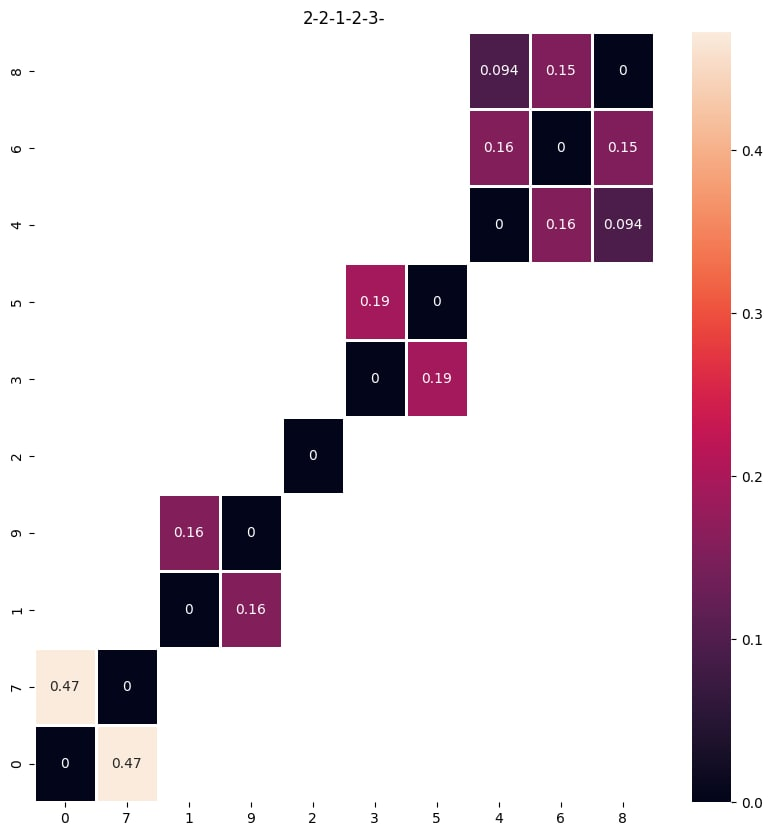
\includegraphics[scale=0.35]{picture1.jpg}}
	\caption{Heatmap with clustered features.}
	\label{fig1}
\end{figure}

\begin{figure}[hbt!]
	\centerline{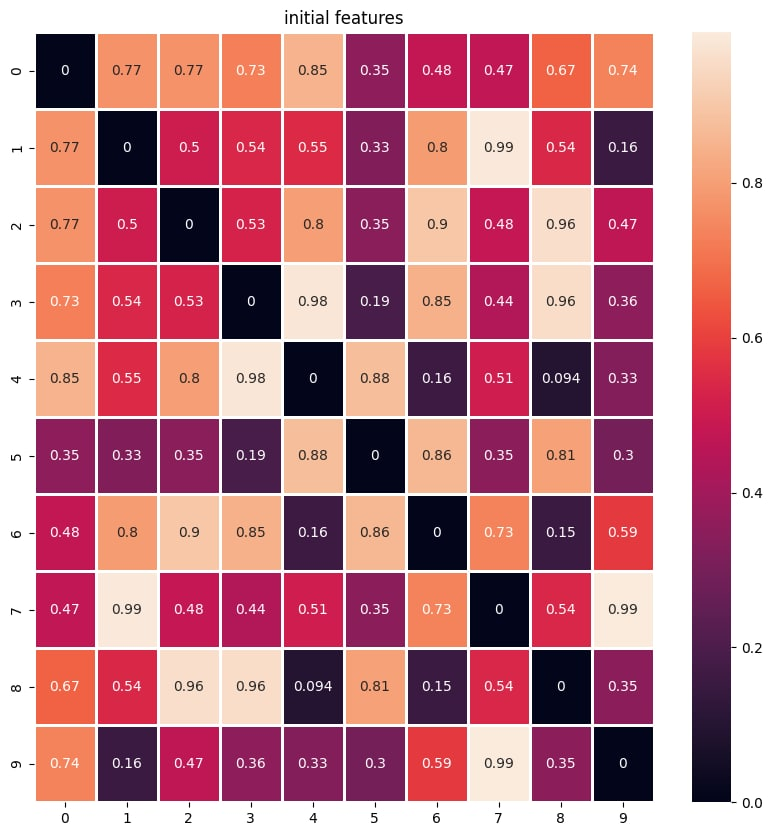
\includegraphics[scale=0.35]{picture2.jpg}}
	\caption{Full heatmap of distances.}
	\label{fig2}
\end{figure}

\begin{equation}
	x_{i, j}=1-spr(i, j)
\end{equation}

The algorithm will be checking the table to find features that are most closely correlated, and grouping them in clusters (Fig. 1), later applying Principal Component Analysis to select one of the features from the cluster to explain the influence of all of them onto the target. Ideally, that would remove the multicollinearity problem, and allow us to reduce the number of features in the dataset without significantly harming the predictive capacity of the model. \\ \\ \\

\begin{lstlisting}[language=Python]{Clustering pseudocode}
for feature in features:
	if feature.VIF > 2.5:
		n.add(feature)
n.compute_correlation_matrix()
n.get_dist_matrix(n.correlation_matrix)
clusters = n.create_clusters(n.dist_matrix)
for cluster in clusters:
	final_feats.add(cluster.apply_pca())
return final_feats
\end{lstlisting}

\subsection{Feature Selection}

In our research, we were able to identify three categories of feature selection methods. Firstly, it is the filter method, which ranks each feature on some statistical metric, and evaluates the ranks afterwards, picking the ones that score the highest. Secondly, it is the wrapper method, which takes a subset of features and trains a model using them. Depending on results of the testing, it adds or removes features from the subset, incrementally improving the performance until user-defined stopping criteria is achieved. Thirdly, it is the embedded method, which is in-built into models themselves - it add a penalizing term to the regression equation (en example of such a model would be Lasso Regression)\cite{twdMLfeatsec}.\\

Among all categories mentioned, wrapper method has the highest computational costs, but can provide the best dataset that would provide the most accurate results for our model. It can also include nature-inspired algorithms as its estimators, making \textbf{wrapped} category of feature selection models our preferred choice.\\

NiaPy library provides many implementations of different nature-inspired algorithms, and using all of them in our project would have been very inefficient. Since we already do most of the preprocessing ourselves and without aid from the evopreprocess library, and use some nature-inspired algorithms in our work (that is, particle swarm optimization and genetic algorithm), we have decided to use another algorithm as an optimizer for the evopreprocess library. The cuckoo search algorithm, that was taught on the most recent lecture, caught our attention, and after finding out that it was already used for feature selection by researchers\cite{aziz2018modified}\cite{rodrigues2013bcs}, we have decided to select it as the optimizer in \texttt{EvoFeatureSelection} class. Levy Flights used in Cuckoo Search are also usually far more efficient than other randomization techniques based on random-walks. It also preserves a high performance while also ranking as the fastest NIC algorithm in feature selection tasks.\cite{karakativc2020evopreprocess}\\ 

\subsection{Feature Transformation}

Another important step in the preprocessing that we designed is feature transformation. It is undeniable that relations between target variables and predictors in real-world data rarely posses two of the most desirable statistical properties:
\begin{itemize}
	\item Data having a normal distribution
	\item Linear relation between target variable and predictors
\end{itemize}
The main goal of this feature engineering step is to apply a number of functions on the given features to map it as much as possible to a normal distribution. Such procedure it likely to improve performance by possibly increase the linear correlation between the independent and dependent variables. Our implementation of this step is highly inspired by TPOT as the it makes use of Genetic Algorithm to find the best ML pipeline.\\

Our solution uses the following transformations:
\begin{itemize}
	\item cox-box
	\item yeo-johnson
	\item Reciprocal
	\item Square root
	\item Quantile transformation (mapping to a uniform distribution)
	\item Polynomial: (from degree 1 up to degree 5)
\end{itemize}

A genetic algorithm is generally defined by: 
\begin{enumerate}
	\item Problem presentation (interpretation of the chromosome data structure)
	\item Genetic operators: crossover, mutation, selection 
	\item Performance evaluation
\end{enumerate}

Denoting by n the number of features,
\begin{itemize}
	\item Our chromosome is a sequence of $n$ genes, where each gene is associated with an integer value. The latter maps to one of the predefined transformations mentioned above. The latter will be applied on the corresponding feature 
	\item Mutation operator: under a predetermined probability (mutation probability), a gene undergoes the following depending on the initial associated transformation: 
	\begin{itemize}
		\item It mapped to a different non-polynomial transformation if it is initially associated with a non-polynomial transformation
		\item If it is initially associated with a polynomial transformation, then its degree either increments or decrements with 0.5 probability
	\end{itemize}
	\item Provided with the target variable, a particle is scored as follows:
	\begin{equation}
		score=\dfrac{\sum_{i=1}^{n}|corr(y, f_i(x_i))|}{n}
	\end{equation}
\end{itemize}

\section{Github link}
\href{https://github.com/Daru1914/NIC\_Project}{https://github.com/Daru1914/NIC\_Project}

\section{Experiments and Evaluation}

While initially the goal of the project was to evaluate the population growth dataset, the goals were expanded to include testing for any unoptimized generic dataset, which is why our testing not only covers the regression models, but also the classification ones.

\subsection{Testing for Elimination of Multicollinearity}

First part of preprocessing that we tested was the removal of multicollinearity with the help of clustering and PSO algorithm. Using modules imported from sklearn, we generated a batch of 100 datasets. Each one was used for classification task with logistic regression, and contained 25 features with 8 informative ones and 6 redundant ones. However, initial implementation of the PSO contained mistakes, and some useful features where removed by the algorithm, because of which the accuracy of predictions in general became significantly worse after preprocessing.\\

After fixing those mistakes, new tests were run. In general model performed much better, as the accuracy no longer fell by 20-30\% percent after the preprocessing, as was the case before. In order to interpret the results of testing more effectively, we have modified the output to include counters of the number of times performance was improved, and the number of times performance has decreased, and ran the output again. The results of that testing showed that:

\begin{table}[htbp]
	\caption{Testing results}
	\begin{center}
		\begin{tabular}{|c|c|c|}
			\hline
			\textbf{Tests number}&\textbf{Increased accuracy}&\textbf{Decreased accuracy} \\
			\hline
			100&16&49\\
			\hline
		\end{tabular}
		\label{tab1}
	\end{center}
\end{table}

From those results it could be concluded that our preprocessing was ineffective and produced too many results with decreased accuracy. However, our testing was also somewhat flawed. One of the main positive consequences of dealing with multicollinearity is removal of useless features, and it wasn't tracked at all during testing. Moreover, manual observation of results of each test showed that in most of the cases where accuracy suffered, it was only reduced by a very small fraction. Keeping those observations in mind, we have redesigned the testing process.\\

We have added the option for the number of informative and redundant features to be generated randomly, and also started tracking the number of features removed with each iteration of the loop. Also, new criteria have been chosen to classify preprocessing as degrading accuracy of predictions - it will only be classified so, if the difference between the accuracy score before and after application of PSO clustering is greater than 0.001. The number of iterations of the testing loop was also reduced from 100 to 25 (execution time of 100 iterations approached 1.5 hours). Results received after the testing was reworked are as follows:

\begin{table}[htbp]
	\caption{Testing for Multicollinearity}
	\begin{center}
		\begin{tabular}{|c|c|c|c|c|}
			\hline
			\textbf{Inf. range}&\textbf{Redund. range}&\textbf{Imp. acc.}&\textbf{Dec. acc.}&\textbf{Avg. rem. feats} \\
			\hline 
			6-9& 4-6& 3& 0& 5.5 \\
			\hline 
			6-9& 4-6& 7& 0& 5.44 \\
			\hline 
			6-10& 4-7& 7& 0& 5.44 \\
			\hline
		\end{tabular}
		\label{tab2}
	\end{center}
\end{table}

Results of the conducted tests confirm our earlier assessment of the effect that PSO clustering has had on the dataset and the multicollinearity problem in particular. It never significantly harms the accuracy of the model and in rare cases even improves it, while also removing more than 20\% of features that are unnecessary and thereby simplifying the work during future preprocessing and prediction. While the increase in performance is not very evident on a fairly small dataset, such as ours, it would be very significant in real-world tasks related to statistical aspects of banking, finance and government.  

\subsection{Transformations testing}

The effect of feature transformations was tested on 3 generated datasets for classification. Each one of them was tested on several classification models, both before and after the observations, and their accuracy score was compared. Said classification models are as follows: 

\begin{enumerate}
	\item K neighbors classifier with 3 neighbors
	\item Linear SVM with $C=0.025$
	\item RBF SVM with $gamma = 2$, $C = 1$
	\item Decision Tree Classifier with $max_depth = 5$
	\item Random Forest Classifier with $10$ estimators, $max_depth=5$, $max_features=1$
\end{enumerate}

The results of that testing are as follows:

\begin{table}[hbt!]
	\caption{Transformations for dataset 0}
	\begin{center}
		\begin{tabular}{|c|c|c|}
			\hline
			\textbf{Model}&\textbf{Accuracy before transf.}&\textbf{Accuracy after transf.} \\
			\hline
			Nearest Neighbors&0.905&0.908125 \\
			\hline
			Linear SVM&0.8675&0.885 \\
			\hline
			RBF SVM&0.918125&0.92125 \\
			\hline
			Decision Tree&0.908125&0.90875 \\
			\hline
			Random Forest&0.91875&0.915625 \\
			\hline
		\end{tabular}
		\label{tab3}
	\end{center}
\end{table}

\begin{table}[hbt!]
	\caption{Transformations for dataset 1}
	\begin{center}
		\begin{tabular}{|c|c|c|}
			\hline
			\textbf{Model}&\textbf{Accuracy before transf.}&\textbf{Accuracy after transf.} \\
			\hline
			Nearest Neighbors&0.85625&0.868125 \\
			\hline
			Linear SVM&0.5375&0.886875 \\
			\hline
			RBF SVM&0.885625&0.889375 \\
			\hline
			Decision Tree&0.8575&0.870625 \\
			\hline
			Random Forest&0.864375&0.8775 \\
			\hline
		\end{tabular}
		\label{tab4}
	\end{center}
\end{table}

\begin{table}[hbt!]
	\caption{Transformations for dataset 2}
	\begin{center}
		\begin{tabular}{|c|c|c|}
			\hline
			\textbf{Model}&\textbf{Accuracy before transf.}&\textbf{Accuracy after transf.} \\
			\hline
			Nearest Neighbors&0.894375&0.888125 \\
			\hline
			Linear SVM&0.906875&0.90875 \\
			\hline
			RBF SVM&0.915625&0.903125 \\
			\hline
			Decision Tree&0.901875&0.89875 \\
			\hline
			Random Forest&0.91625&0.90625 \\
			\hline
		\end{tabular}
		\label{tab4}
	\end{center}
\end{table}

As we can see, feature transformation produced small improvements in accuracy, when accuracy for the initial dataset was high enough, and it produced a major increase in it when accuracy was low (Linear SVM for dataset 1). However, in the testing of the last dataset (which was the most complicated), the feature transformation actually decreased the accuracy by a small amount. Generally this type of dataset can be separated by applying kernel transformations and functions such as RBF. \\

\subsection{Testing the preprocessing pipeline}

Testing of the population growth dataset on the entire preprocessing pipeline was performed using several selected regression models, that is: Ridge, Lasso, Decision Tree, KNN, Random Forest regressions. We have given the initial dataset to all aforementioned models and done the same thing after putting the dataset through our preprocessing pipeline. Though our implementation allows for a choice of many different metrics to compare the performance of the models, we have decided to stick to the mean square error (MSE). Results of our testing are given below:

\begin{table}[htbp]
	\caption{Pipeline testing}
	\begin{center}
		\begin{tabular}{|c|c|c|}
			\hline
			\textbf{Model}&\textbf{Pre-pipeline MSE}&\textbf{Post-pipeline MSE}\\
			\hline
			Ridge&0.179&0.818 \\
			\hline
			Lasso&0.179&1.264 \\
			\hline
			Decision Tree&0.676&0.791 \\
			\hline
			K Neighbors&0.133&0.298 \\
			\hline
			Random Forest&0.448&0.580 \\
			\hline
		\end{tabular}
		\label{tab1}
	\end{center}
\end{table}

\section{Analysis and Observations}

The previous section covers in details the results of our experimental attempt. The different pipeline components achieved reasonable performance on the toy datasets generated by tools such as scikit-learn. It is crucial to  bear in mind that those datasets are indeed of limited complexity and do not introduce complex and non-linear interactions between the predictors and the target variable.\\

The comparison of the performance of Machine Learning models before and after applying the transformation further justifies this claim. (refer to Fig. 3). 

\begin{figure}[hbt!]
	\centerline{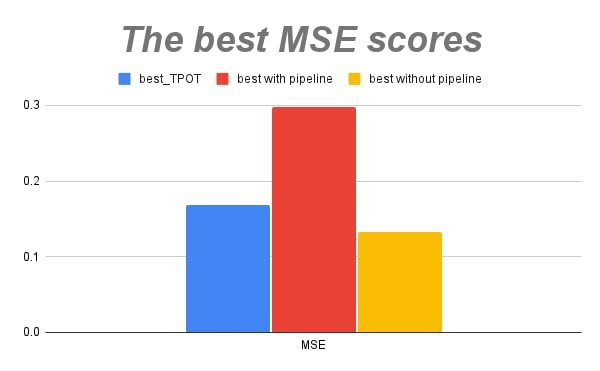
\includegraphics[scale=0.55]{picture3.jpg}}
	\caption{Best MSE scores.}
	\label{fig1}
\end{figure}

The current implementation is indeed limited and not suitable to tackle such a difficult challenge (building a NIC-based preprocessing pipeline) with complex and high-dimentional real-world data. \\

Nevertheless, we believe that the overall performance, in the light of the limited experience, the experimental nature of the project and the time constraints, is quite satisfactory.


\section{Conclusion}

In the end, while our preprocessing pipeline has not managed to improve accuracy of the predictions in comparison to just operating on the given dataset, the drop in accuracy was not significant, and we have managed to rid the dataset of several mostly redundant features in the process. \\

However, the room for improvement is quite large with the current implementation. The following upgrades deserve consideration:
\begin{itemize}
	\item Building more mathematically-robust scoring functions instead of determining it on experimental basis
	\item Conceive better techniques to link between the discrete nature of the problem and the continuous nature of the optimization algorithms
	\item Applying more rigorous statistical analysis, as well as considering additional datasets
\end{itemize}

\bibliographystyle{plain}
\bibliography{referens}

\end{document}
